\documentclass[12pt,a4]{article}
\usepackage[]{graphicx}\usepackage[]{xcolor}
% maxwidth is the original width if it is less than linewidth
% otherwise use linewidth (to make sure the graphics do not exceed the margin)
\makeatletter
\def\maxwidth{ %
  \ifdim\Gin@nat@width>\linewidth
    \linewidth
  \else
    \Gin@nat@width
  \fi
}
\makeatother

\definecolor{fgcolor}{rgb}{0.345, 0.345, 0.345}
\newcommand{\hlnum}[1]{\textcolor[rgb]{0.686,0.059,0.569}{#1}}%
\newcommand{\hlstr}[1]{\textcolor[rgb]{0.192,0.494,0.8}{#1}}%
\newcommand{\hlcom}[1]{\textcolor[rgb]{0.678,0.584,0.686}{\textit{#1}}}%
\newcommand{\hlopt}[1]{\textcolor[rgb]{0,0,0}{#1}}%
\newcommand{\hlstd}[1]{\textcolor[rgb]{0.345,0.345,0.345}{#1}}%
\newcommand{\hlkwa}[1]{\textcolor[rgb]{0.161,0.373,0.58}{\textbf{#1}}}%
\newcommand{\hlkwb}[1]{\textcolor[rgb]{0.69,0.353,0.396}{#1}}%
\newcommand{\hlkwc}[1]{\textcolor[rgb]{0.333,0.667,0.333}{#1}}%
\newcommand{\hlkwd}[1]{\textcolor[rgb]{0.737,0.353,0.396}{\textbf{#1}}}%
\let\hlipl\hlkwb

\usepackage{framed}
\makeatletter
\newenvironment{kframe}{%
 \def\at@end@of@kframe{}%
 \ifinner\ifhmode%
  \def\at@end@of@kframe{\end{minipage}}%
  \begin{minipage}{\columnwidth}%
 \fi\fi%
 \def\FrameCommand##1{\hskip\@totalleftmargin \hskip-\fboxsep
 \colorbox{shadecolor}{##1}\hskip-\fboxsep
     % There is no \\@totalrightmargin, so:
     \hskip-\linewidth \hskip-\@totalleftmargin \hskip\columnwidth}%
 \MakeFramed {\advance\hsize-\width
   \@totalleftmargin\z@ \linewidth\hsize
   \@setminipage}}%
 {\par\unskip\endMakeFramed%
 \at@end@of@kframe}
\makeatother

\definecolor{shadecolor}{rgb}{.97, .97, .97}
\definecolor{messagecolor}{rgb}{0, 0, 0}
\definecolor{warningcolor}{rgb}{1, 0, 1}
\definecolor{errorcolor}{rgb}{1, 0, 0}
\newenvironment{knitrout}{}{} % an empty environment to be redefined in TeX

\usepackage{alltt}
\newcommand{\SweaveOpts}[1]{}  % do not interfere with LaTeX
\newcommand{\SweaveInput}[1]{} % because they are not real TeX commands
\newcommand{\Sexpr}[1]{}       % will only be parsed by R



% ---- Metadata ---- %

\title{Honesty by Convenience: Corruption Tolerance in Ecuador}
\author{Daniel Sánchez}
\date{June 2022}

% ---- Load Packages ---- %

% Math

\usepackage{savesym} % Need to "save" the command that is already defined \varTheta

\usepackage{amsmath}
  \savesymbol{varTheta} 

% Fonts

% To set the TNR font for both text and equations:

\usepackage{mathspec}
  \setallmainfonts(Digits,Greek,Latin){Times New Roman}
\restoresymbol{MTP}{varTheta}

% Formatting

\usepackage{setspace}
  \doublespacing

\usepackage[margin = 1in]{geometry}

\usepackage{lscape}

% Setting the size of the section titles

\usepackage{titlesec}

\titleformat*{\section}{\normalsize\bfseries}

% Citation & Bibliographies

\usepackage[backend = biber, style = apa, citestyle = apa]{biblatex}
  \addbibresource{refs.bib}
  
% For tables:

 % For the modelsummary tables:
\usepackage{siunitx}
\usepackage{booktabs} 
  \newcolumntype{d}{S[input-symbols = ()]}
\usepackage{multirow}
\usepackage[flushleft]{threeparttable}

% For figure and table captions

\usepackage{caption}
  \captionsetup{labelfont = bf} % All in bold  
  
% Other packages

\usepackage{csquotes} % For quotation marks

\usepackage{epigraph} % For epigraph
  \setlength\epigraphwidth{9cm}
  \setlength\epigraphrule{1pt}

\usepackage{float} % For the H float option- only used in emergencies (lol)

\usepackage{textcomp} % For the registered trademark symbol.

% Always load these packages at the end of the preamble:

\usepackage{hyperref}

% ---- R Stuff to be used in the whole document ----

% Here I will execute or source R code through chunks that I need to use throughout the whole document.

% General settings



% Load the data by sourcing the data manipulation script. Note that survey design objects are indeed created in this script.
% We use the time argument in the chunks to reread or rerun the chunk in case external files are updated and chunks need to be rerun and re-cached.


% Perform all survey-robust tabulations by sourcing the R Script. 
% These are used on the text later.





\begin{document}
% Context .Rnw File

\section{Institutional and Historical Background}
\label{sec:background}

As pointed out previously, the corruption tolerance increase happened at the same time as other key events. First, AB indicators denote a political crisis, as support for President Rafael Correa's regime took a sharp hit. Second, a recession hit Ecuador due to a commodity price collapse, an earthquake and other circumstances. Below, Figure \ref{fig:ecua_pol} shows several public opinion indicators and Figure \ref{fig:ecua_ec} displays economic conditions, both observed and perceived from 2014 to 2019. 
% Create the data to be used for the political opinion variables:

% Now do the graph
\begin{figure}[htbp]
\centering
\fbox{
\begin{minipage}{\textwidth}
\caption{Ecuadorian public opinion indicators, 2004-2019}
\label{fig:ecua_pol}
\begin{knitrout}
\definecolor{shadecolor}{rgb}{0.969, 0.969, 0.969}\color{fgcolor}

{\centering 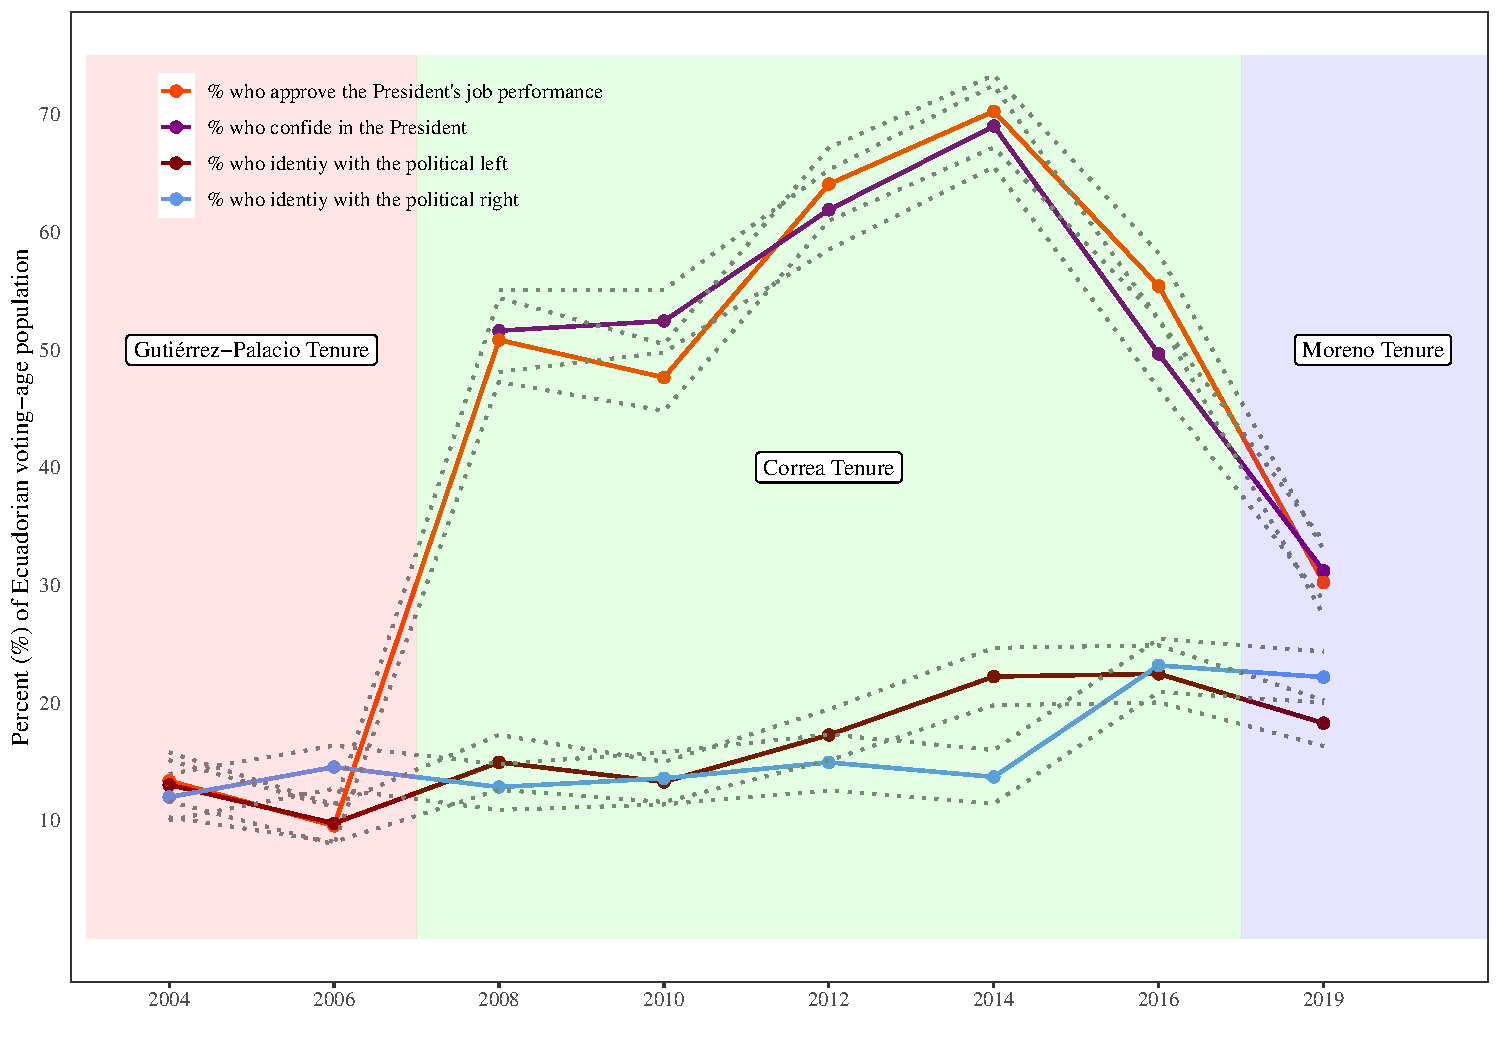
\includegraphics[width=\maxwidth]{figure/political_graph-1} 

}


\end{knitrout}
\textbf{Note:} The graph shows time series for political public opinion questions asked in the AB. Percentages are estimated as explained in \hyperref[app:first]{Appendix A} and error bars show 95\% confidence intervals considering design effects. Figure prepared by the author. \end{minipage}
}
\end{figure}

The AB data shows that indeed the President reached an all-time high popularity in 2014 and then a severe drop in 2016. This is seen through the percent of people who approve the President's job performance and the percent who report confidence in him. Another notable change in the political landscape is the way that voting-age population politically identified. There was a strong increase of the people who identified as the \enquote{right}, while those who identified with the \enquote{left} did not see significant changes.

Regarding the economic recession, \textcite{Orozco.2015} holds that although the commodity price collapse in 2008 was greater, there was little reduction in economic activity as the country had greater possibilities of international financing and savings left over from past oil funds, which were used to keep government expenditure high. In 2016, as savings eroded and government debt had grown bigger, the economy stagnated significantly for the first time in the Correa administration. Combined with the lack of competitiveness in exports due to US dollar appreciations and the poor public finance administration \parencite{Hurtado.2018}, the country fell into a deep economic recession. While the official GDP figures may show only a small reduction in GDP growth, \textcite{Hurtado.2018} holds that these figures are overestimated.

% Here I create my graph, but I need to load some libraries first and create the data needed for my graphs.

% Now I do the graph:
\begin{figure}[htbp]
\begin{center}
\fbox{
\begin{minipage}{\textwidth}
\caption{Ecuadorian economic conditions 2004-2019}
\label{fig:ecua_ec}
\begin{knitrout}
\definecolor{shadecolor}{rgb}{0.969, 0.969, 0.969}\color{fgcolor}

{\centering 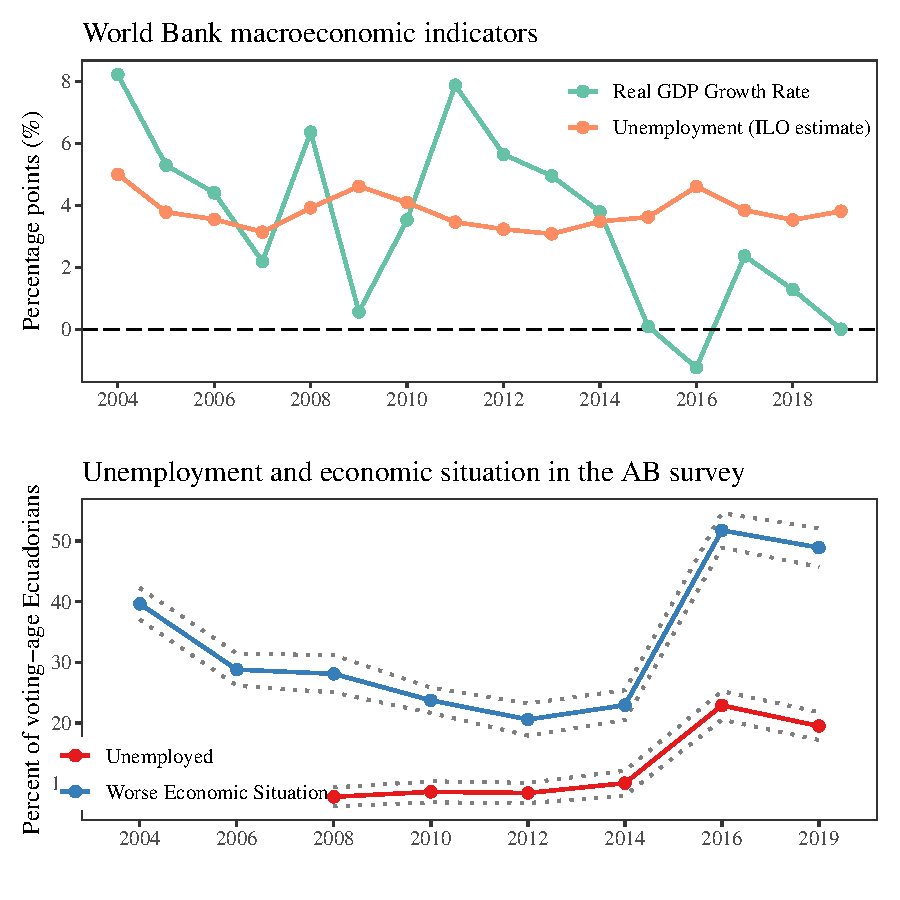
\includegraphics[width=\maxwidth]{figure/econ_graph-1} 

}


\end{knitrout}
\textbf{Note:} Time series line graphs showing key economic indicators for the country between 2004 and 2019. Real GDP growth and unemployment rates extracted from the World Bank's World Development Indicators. WTI oil barrel prices extracted from FRED. The rest are estimates computed with the open-access AB databases, which include 95\% confidence intervals adjusted for design effects. See \hyperref[app:first]{Appendix A} for details on calculations. Figure prepared by the author. 
\end{minipage}}
\end{center}
\end{figure}

Figure \ref{fig:ecua_pol} shows several indicators of public opinion in the country. The AB data shows that indeed the President reached an all-time high popularity in 2014 and then a severe drop in 2016. This is seen through the percent of people who approve the President's job performance and the percent who report confidence in him. Another notable change in the political landscape of this period is the way that voting-age population identified politically. There was a notable increase of the people who identified as the \enquote{right} of the political wings, while those who identified with the \enquote{left} did not see significant changes.
\end{document}
